%\input{/Users/joshyv/Research/misc/latex_paper.tex}
\documentclass{article}
\usepackage{amsmath}
\usepackage{graphicx}
\usepackage{amsfonts}
\usepackage{amssymb}
\usepackage{amsthm}
%\usepackage{cite}
\usepackage{algorithm}
\usepackage{algorithmic}
% \usepackage{times}
\usepackage{fancyhdr}
\usepackage{graphicx}
\usepackage{verbatim}
\usepackage{color}
\usepackage[T1]{fontenc}
\usepackage[scaled]{helvet}
\renewcommand*\familydefault{\sfdefault} %% Only if the base font of the document is to be sans serif
\pagestyle{fancy}

\oddsidemargin=0.0in %%this makes the odd side margin go to the default of 1inch
\evensidemargin=0.0in
\textwidth=6.5in
\headwidth=6.5in
\textheight=9in %%sets the textwidth to 6.5, which leaves 1 for the remaining right margin with 8 1/2X11inch paper
\headheight=12pt
\topmargin=-0.25in
%\headheight=0in
%\headsep=0in
%\pagestyle{headings}

\usepackage{hyperref}
% \usepackage{ulem}
% \usepackage{color}

% \newcommand{\loo}{$L^{(1)}_{h; \mD_n}$}
\newcommand{\conv}{\rightarrow}
% \newcommand{\Real}{\mathbb{R}}
% \providecommand{\tr}[1]{\textcolor{red}{#1}}

\newcommand{\mB}{\mathcal{B}}
\newcommand{\mD}{\mathcal{D}}
\newcommand{\mM}{\mathcal{M}}
\newcommand{\PP}{F}           % probability
\newcommand{\EE}{\mathbb{E}}           % expected value
\newcommand{\II}{\mathbb{I}}           % expected value
\newcommand{\Real}{\mathbb{R}}           % expected value

\newcommand{\del}{\delta}
\newcommand{\sig}{\sigma}
\newcommand{\lam}{\lambda}
\newcommand{\gam}{\gamma}
\newcommand{\eps}{\varepsilon}

\providecommand{\mc}[1]{\mathcal{#1}}
\providecommand{\mb}[1]{\boldsymbol{#1}}
\providecommand{\mbb}[1]{\mathbb{#1}}
\providecommand{\mv}[1]{\vec{#1}}
\providecommand{\mh}[1]{\widehat{#1}}
\providecommand{\mt}[1]{\widetilde{#1}}
\providecommand{\mhc}[1]{\hat{\mathcal{#1}}}
\providecommand{\mhb}[1]{\hat{\boldsymbol{#1}}}
\providecommand{\mvb}[1]{\vec{\boldsymbol{#1}}}
\providecommand{\mtb}[1]{\widetilde{\boldsymbol{#1}}}

\newcommand{\argmax}{\operatornamewithlimits{argmax}}
\newcommand{\argmin}{\operatornamewithlimits{argmin}}


% \newcommand{\mN}{\mathcal{N}}

\newcommand{\hL}{\widehat{L}}
\newcommand{\MeB}{\mM \overset{\varepsilon}{{\sim}}_{\PP} \mB}
\newcommand{\MsB}{\mM \overset{S}{\sim}_{\PP} \mB}
\newcommand{\MnoteB}{\mM \overset{\varepsilon}{{\not\sim}}_{\PP} \mB}
\providecommand{\tr}[1]{\textcolor{black}{#1}}
\providecommand{\norm}[1]{\left \lVert#1 \right  \rVert}
\newcommand{\T}{^{\ensuremath{\mathsf{T}}}}           % transpose

\newtheorem{defi}{Definition}
\newtheorem{thm}{Theorem}
\newtheorem{thex}{\emph{Gedankenexperiment}}
\lhead{Vogelstein JT, et al.}
\rhead{Statistical Supervenience Supplement}


\begin{document}

	\begin{center}
{\huge	Supplementary Materials for: \\ Are mental properties supervenient on brain properties?}
\end{center}

\vspace{5px}

% \begin{center}
% {\large		
% Joshua T. Vogelstein$^{1*}$, R. Jacob Vogelstein$^2$, Carey E. Priebe$^1$\\
% 	$^1$Department of Applied Mathematics \& Statistics, \\ Johns Hopkins University, Baltimore, MD, 21218,\\ $^2$National Security Technology Department, \\ Johns Hopkins University Applied Physics Laboratory, Laurel, MD 20723}	
% \end{center}
% 
% \vspace{5px}
% 




% \section{Relations between sets} % (fold)
% \label{sec:relations}

In this appendix we compare supervenience to several other relations on sets (see Figure \ref{fig:rel}).

% aim to provide more intuition regarding supervenience by discussing the limitations and extent of its implications. 

%For instance, it may be the case that minds supervene on brains, but one cannot form an \emph{injective} relation from brains to minds.  

First, a supervenient relation does not imply an injective relation.  An injective relation is any relation that preserves distinctness.  Thus if minds are injective on brains, then $b\neq b' \implies m \neq m'$ (note that the directionality of the implication has been switched relative to supervenience). However, it might be the case that a brain could change without the mind changing.  Consider the case that a single subatomic particle shifts its position by a Plank length, changing brain state from $b$ to $b'$.  It is possible (likely?) that the mental state supervening on brain state $b$ remains $m$, even after $b$ changes to $b'$.  In such a scenario, the mind might still supervene on the brain, but the relation from brains to minds is not injective. This argument also shows that supervenience is not necessarily a \emph{symmetric} relation.  Minds supervening on brains does not imply that brains supervene on minds.  


Second,  supervenience does not imply causality. %it may be the case that minds supervene on brains, but that brains do not cause minds.  
For instance, consider an analogy where $M$ and $B$ correspond to two coins being flipped, each possibly landing on heads or tails.  Further assume that every time one lands on heads so does the other, and every time one lands on tails, so do the other. This implies that $M$ supervenes on $B$, but assumes nothing about whether $M$ causes $B$, or $B$ causes $M$, or some exogenous force causes both.  

Third, supervenience does not imply identity.  The above example with the two coins demonstrates this, as the two coins are not the same thing, even if one has perfect information about the other.  

What supervenience does imply, however, is the following.   Imagine finding two unequal minds.  If $\MsB$, then the brains on which those two minds supervene must be different.  In other words, there cannot be two unequal minds, either of which could supervene on a single brain.  Figure \ref{fig:rel} shows several possible relations between the sets of minds and brains.


Note that statistical supervenience is distinct from statistical correlation.  \emph{Statistical correlation} between brain states and mental states is defined as $\rho_{MB}=\EE[(B-\mu_B)(M-\mu_M)]/(\sig_B \sig_M)$, where $\mu_X$ and $\sig_X$ are the mean and variance of $X$, and $\EE[X]$ is the expected value of $X$.  If $\rho_{MB}=1$, then both $\MsB$ and $\mB \overset{S}{{\sim}}_{F} \mM$. Thus, perfect correlation implies supervenience, but supervenience does not imply correlation.  In fact, supervenience may be thought of as a generalization of correlation which incorporates directionality, can be applied to arbitrary valued random variables (such as mental or brain properties), can depend on any moment of a distribution (not just the first two).


\begin{figure}[h!tbp]
	\centering
		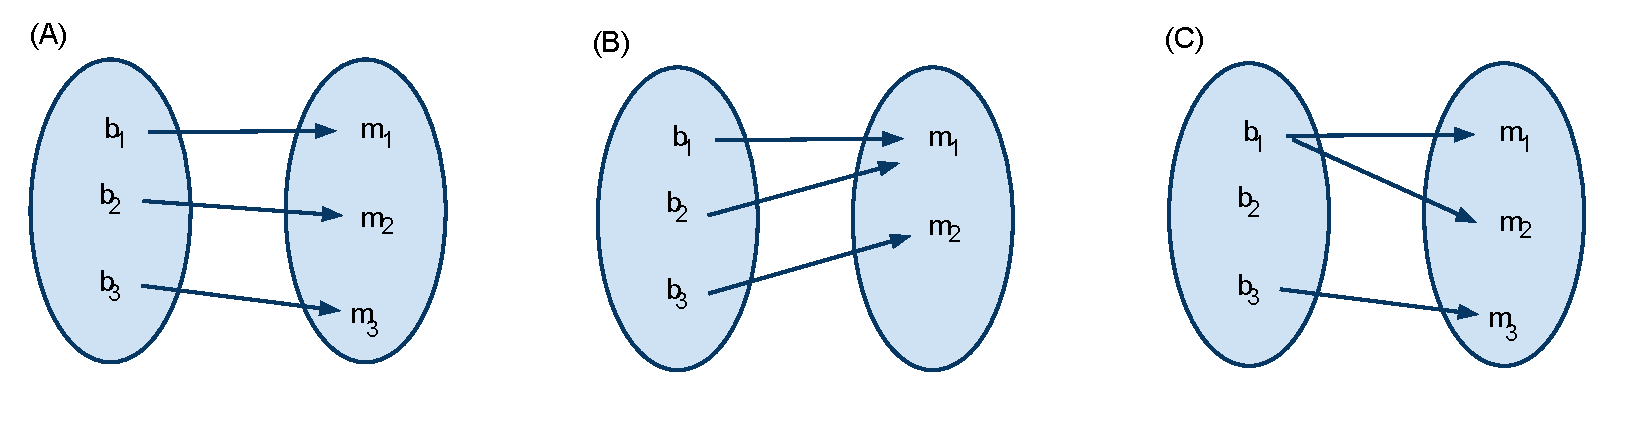
\includegraphics[width=1\linewidth]{supervenience_relations.pdf}
	\caption{Possible relations between minds and brains.  (A) Minds supervene on brains, and it so happens that there is a bijective relation from brains to minds.  (B) Minds supervene on brains, and it so happens that there is a surjective (a.k.a., onto) relation from brains to minds, but not a bijective one. (C) Minds are \emph{not} supervenient on brains, because two different minds supervene on the same brain.}
	\label{fig:rel}
\end{figure}
% section relations_between_sets (end)



% \section{Simulation} % (fold)
% \label{sec:sim}


% \bibliography{/Users/jovo/Research/latex/library}
% \bibliographystyle{nature}



\end{document}

